As launch service providers continue to offer more ride-sharing opportunities, access to space has never been more available or affordable for small satellites. The nanosatellite size (1-10 kg) has exploded in popularity over recent years \citep{NanosatsEU}, and among that size class, the CubeSat has become the de facto standard, as shown in Figure \ref{fig:CubeSat Launches}. A CubeSat is a sizing standard defined in 1999 by California Polytechnic State University and Stanford University's \abbreviationFull[Space and Systems Development Laboratory]{SSDL}, with a basic "1U" unit being 10 cm x 10 cm x 10 cm and a mass less than 1.33 kg \citep{DesignSpec}. A 1U CubeSat is shown in Figure \ref{fig:1U CubeSat Example} for reference, and CubeSats are defined by how many of these 1U cubes they contain. For example, a 3U CubeSat is three 1U cubes together, and a 6U CubeSat is six 1U cubes combined, as shown in Figure \ref{fig:6U CubeSat Example}. Figure \ref{fig:CubeSat Sizes} shows the distribution of sizes, with 1U, 3U, and 6U being the most commonly launched sizes \citep{NanosatsEU}. This standardized sizing framework allows for rapid prototyping with common chassis and common dispenser mechanisms, and this drives down the cost of research and development for these CubeSats. CubeSats also routinely use \abbreviationFull[Commercial Off The Shelf]{COTS} components to further drive down development costs. To assist design teams, California Polytechnic Institute publishes these CubeSat Design Specifications for 1U-3U CubeSats and for 6U CubeSats \citep{DesignSpec}, and NASA publishes a helpful developer's guide called the "CubeSat 101" \citep{NASA101}.

\begin{figure}[H]
    \centering
    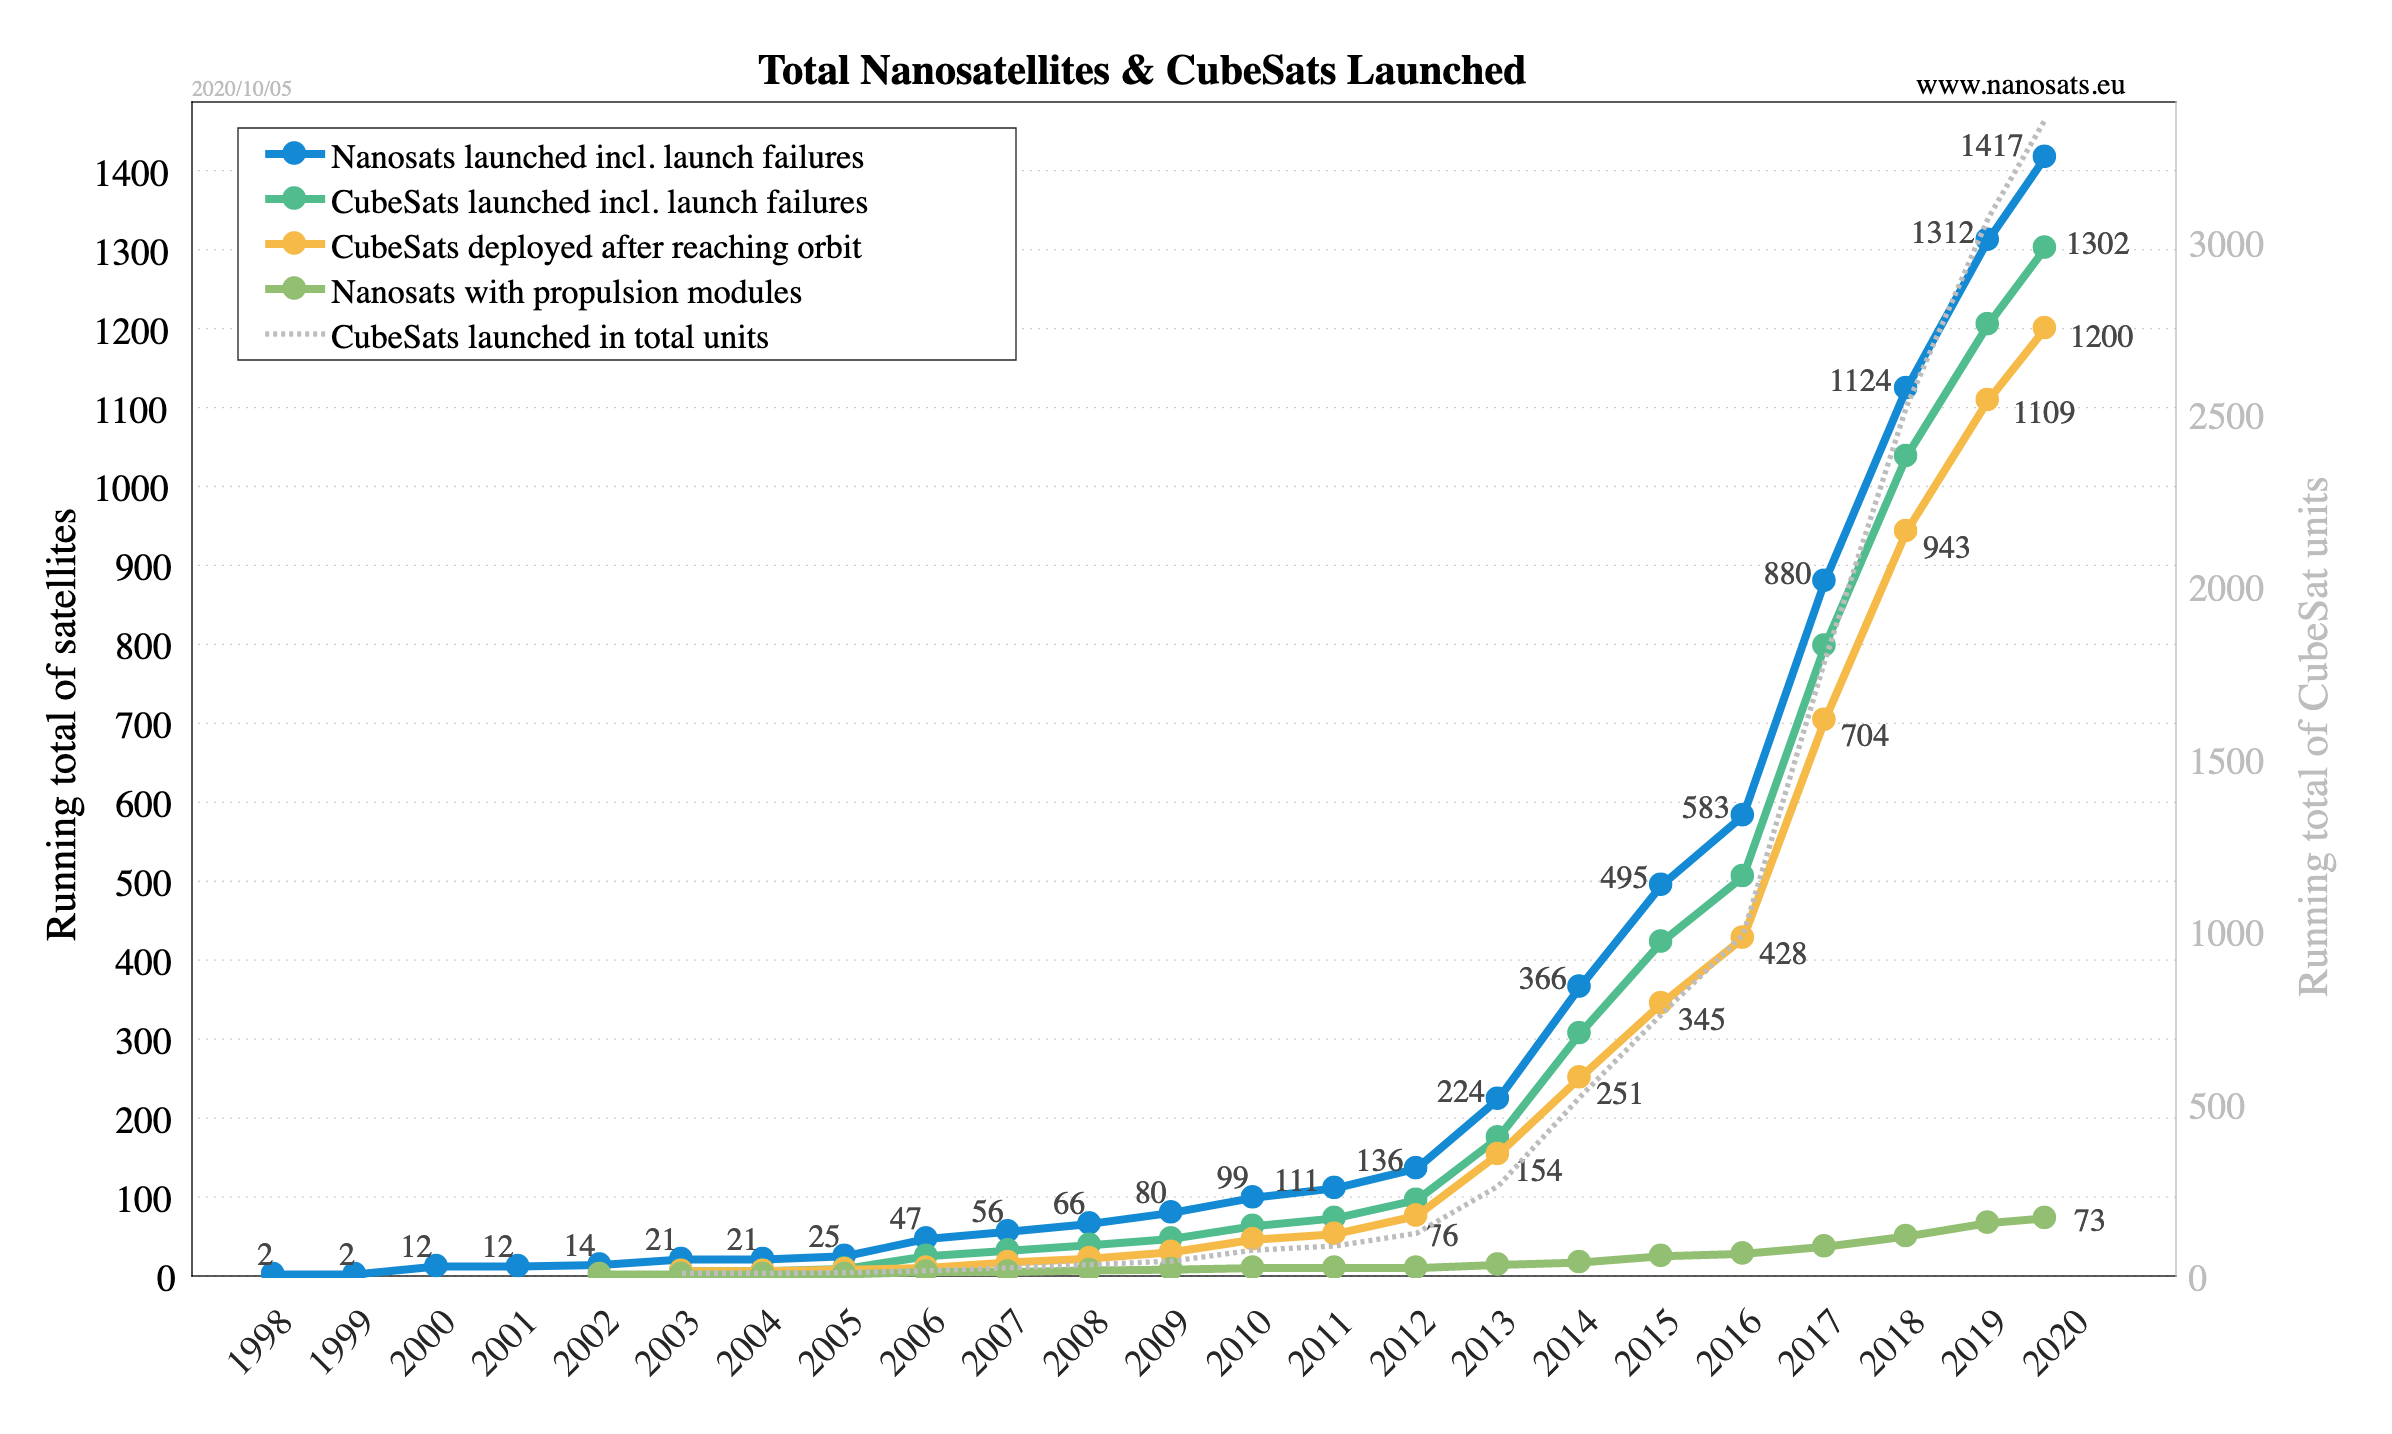
\includegraphics[width=\textwidth]{Thesis/Literature_Review/Lit Review Figures/total launched.png}
    \caption{CubeSat Launches}
    \label{fig:CubeSat Launches}
\end{figure}

\begin{figure}[H]
    \centering
    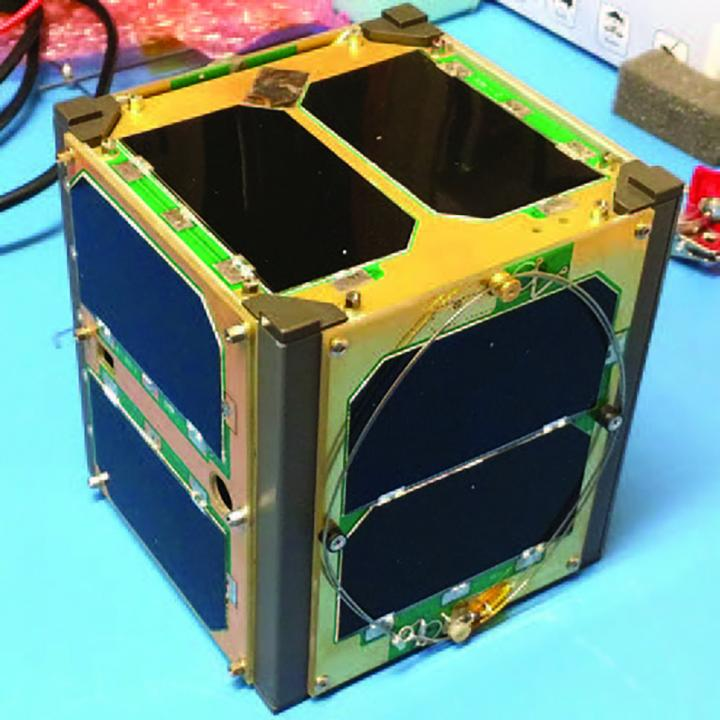
\includegraphics[width=3in]{Thesis/Literature_Review/Lit Review Figures/vanderbiltcubesat.jpg}
    \caption{1U CubeSat Example}
    \label{fig:1U CubeSat Example}
\end{figure}

\begin{figure}[H]
    \centering
    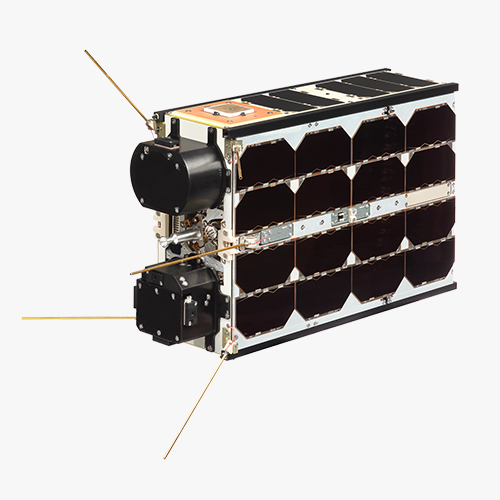
\includegraphics[width=3in]{Thesis/Literature_Review/Lit Review Figures/6Ucubesatbus.jpg}
    \caption{6U CubeSat Example}
    \label{fig:6U CubeSat Example}
\end{figure}

\begin{figure}[H]
    \centering
    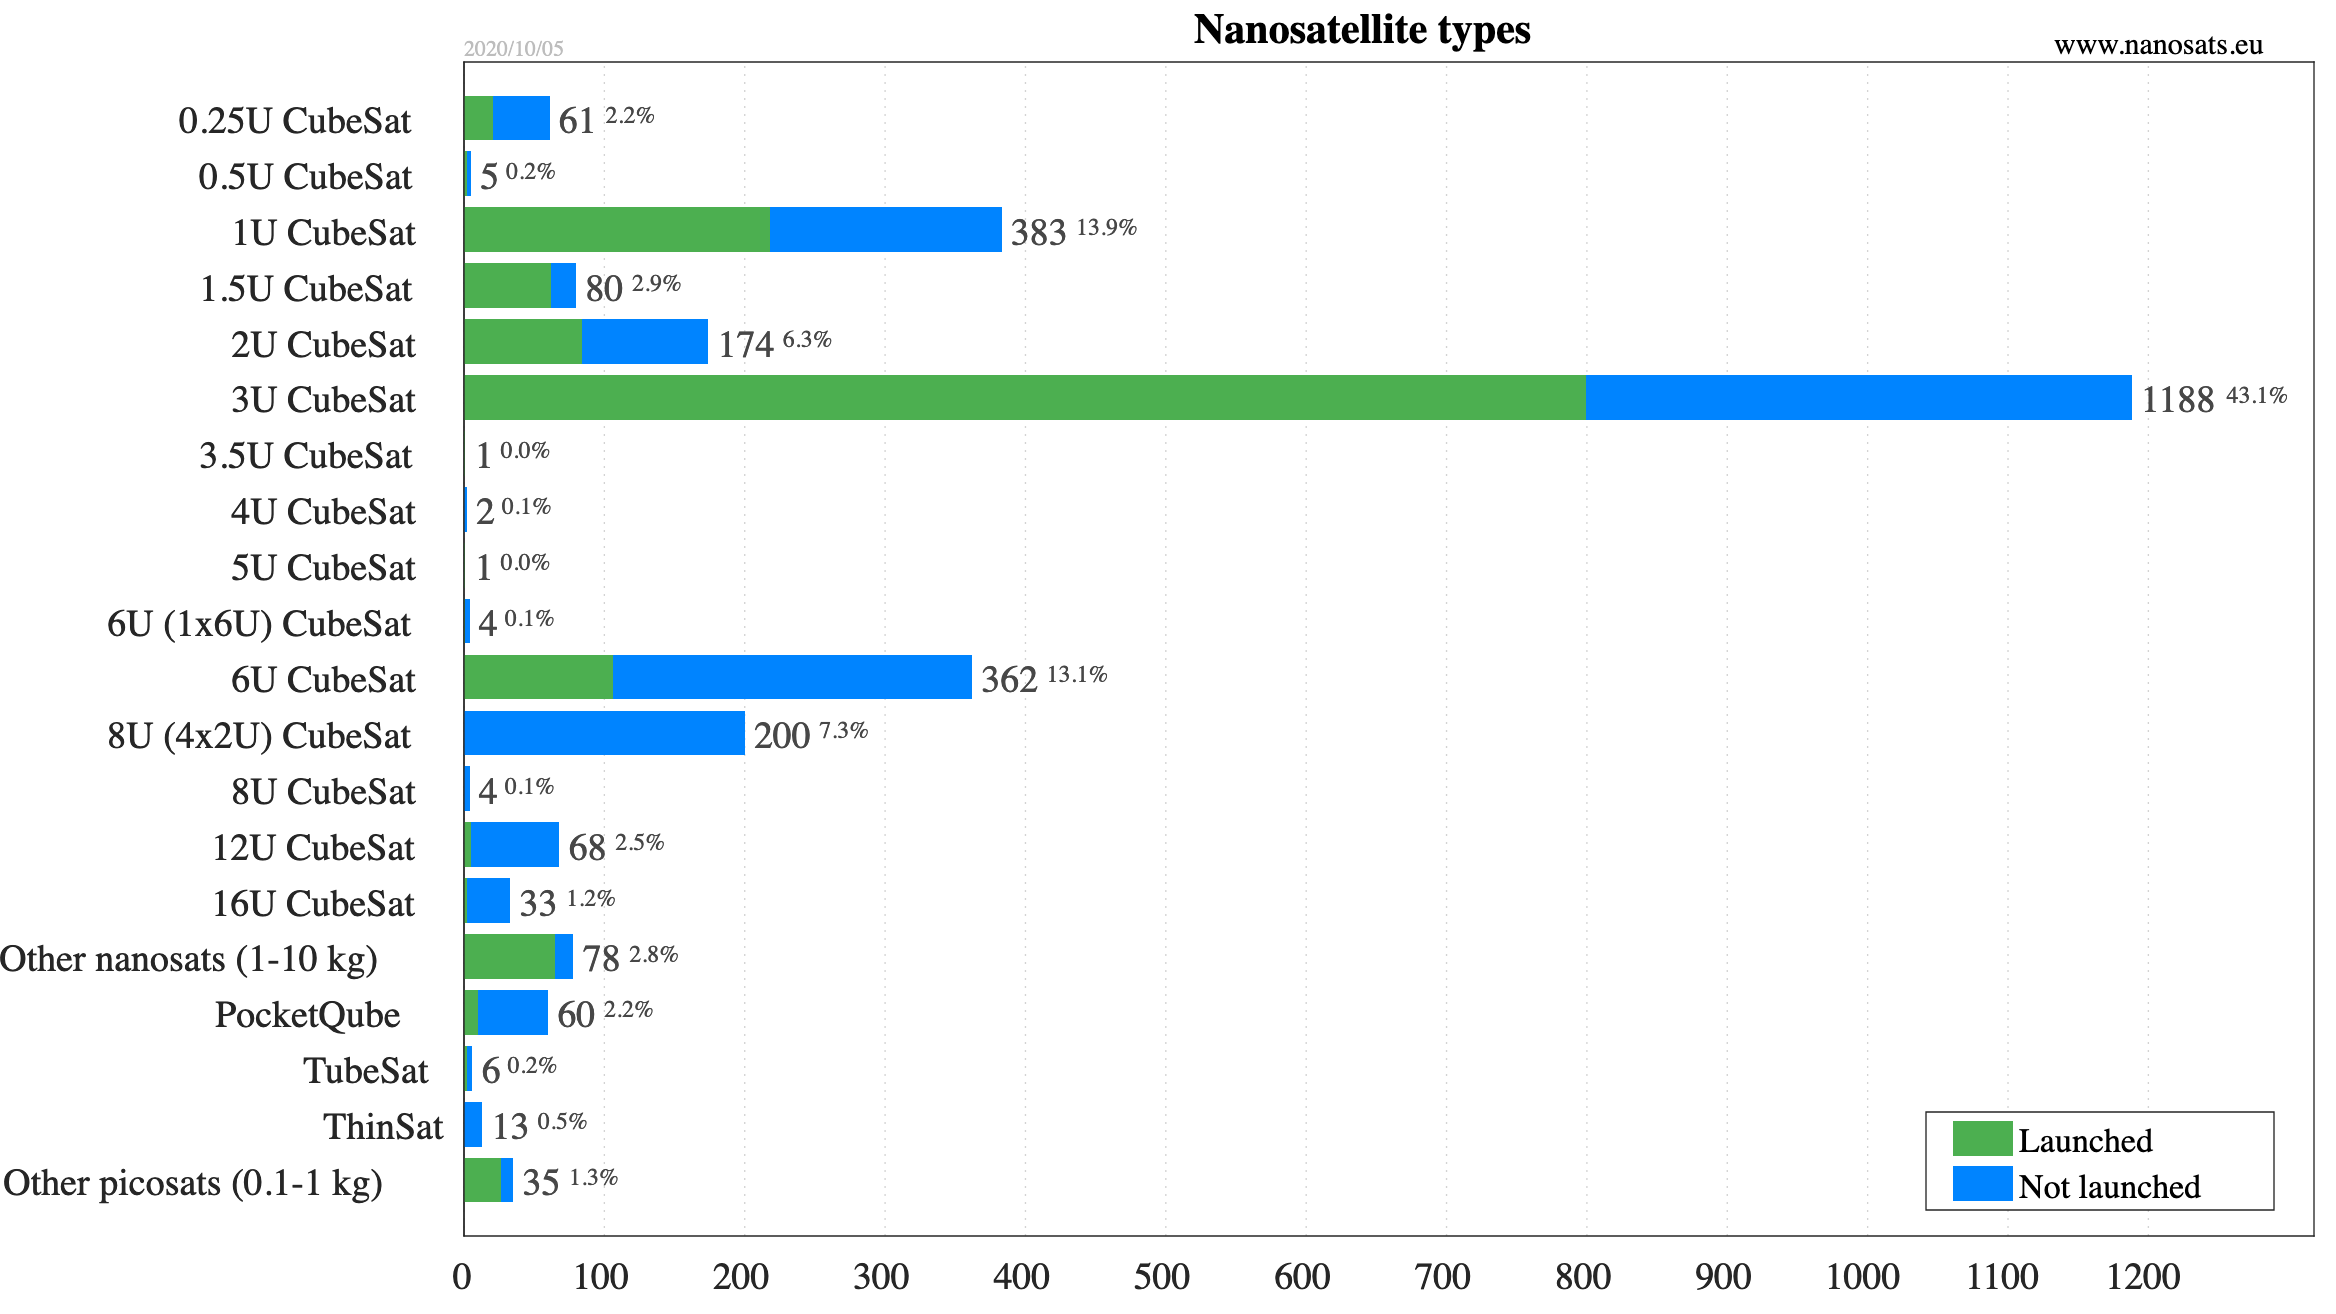
\includegraphics[width=\textwidth]{Thesis/Literature_Review/Lit Review Figures/CubeSat Sizes.png}
    \caption{CubeSat Sizes}
    \label{fig:CubeSat Sizes}
\end{figure}

A primary benefit of the CubeSat standard is the lower cost of both the satellite hardware and launch costs. The cost of failure for a CubeSat is orders of magnitude lower than for a large, exquisite satellite, so CubeSats offer a proving ground for maturing technologies and educating engineers and scientists. A traditional satellite requires a dedicated launch vehicle, a distinct payload adapter, and millions to billions of dollars in research and development. By contrast, a CubeSat might only cost \$100,000 to \$500,000 in research and development costs, and the launch cost can be less than \$1 Million \citep{Wertz2011SpaceSMAD}. Perhaps even more valuable than the reduced cost is the ability to flight test articles in the space environment to iterate and mature technologies. Many materials, sensors, and other components have been matured through CubeSats. For example, the Air Force Academy's FalconSat-7 was designed to record data on a polyimide photon sieve and determine its imaging performance before being used in future operational satellites \citep{FalconSat7}. Their previous mission, FalconSAT-6, was designed to improve \abbreviationFull[Hall Effect Thruster]{HET} technologies and low power communication options \citep{FalconSat6}. CubeSats are an ideal research platform, so it makes sense that Universities launch a significant percentage of total CubeSats, as shown in Figure \ref{fig:CubeSat Development by Institution}, followed by companies seeking to capitalize on this lower-cost launch capability. Figure \ref{fig:CubeSat Companies} shows the drastic increase in new companies developing CubeSats, highlighting the increased relevance of this small satellite size \citep{NanosatsEU}.

\begin{figure}[H]
    \centering
    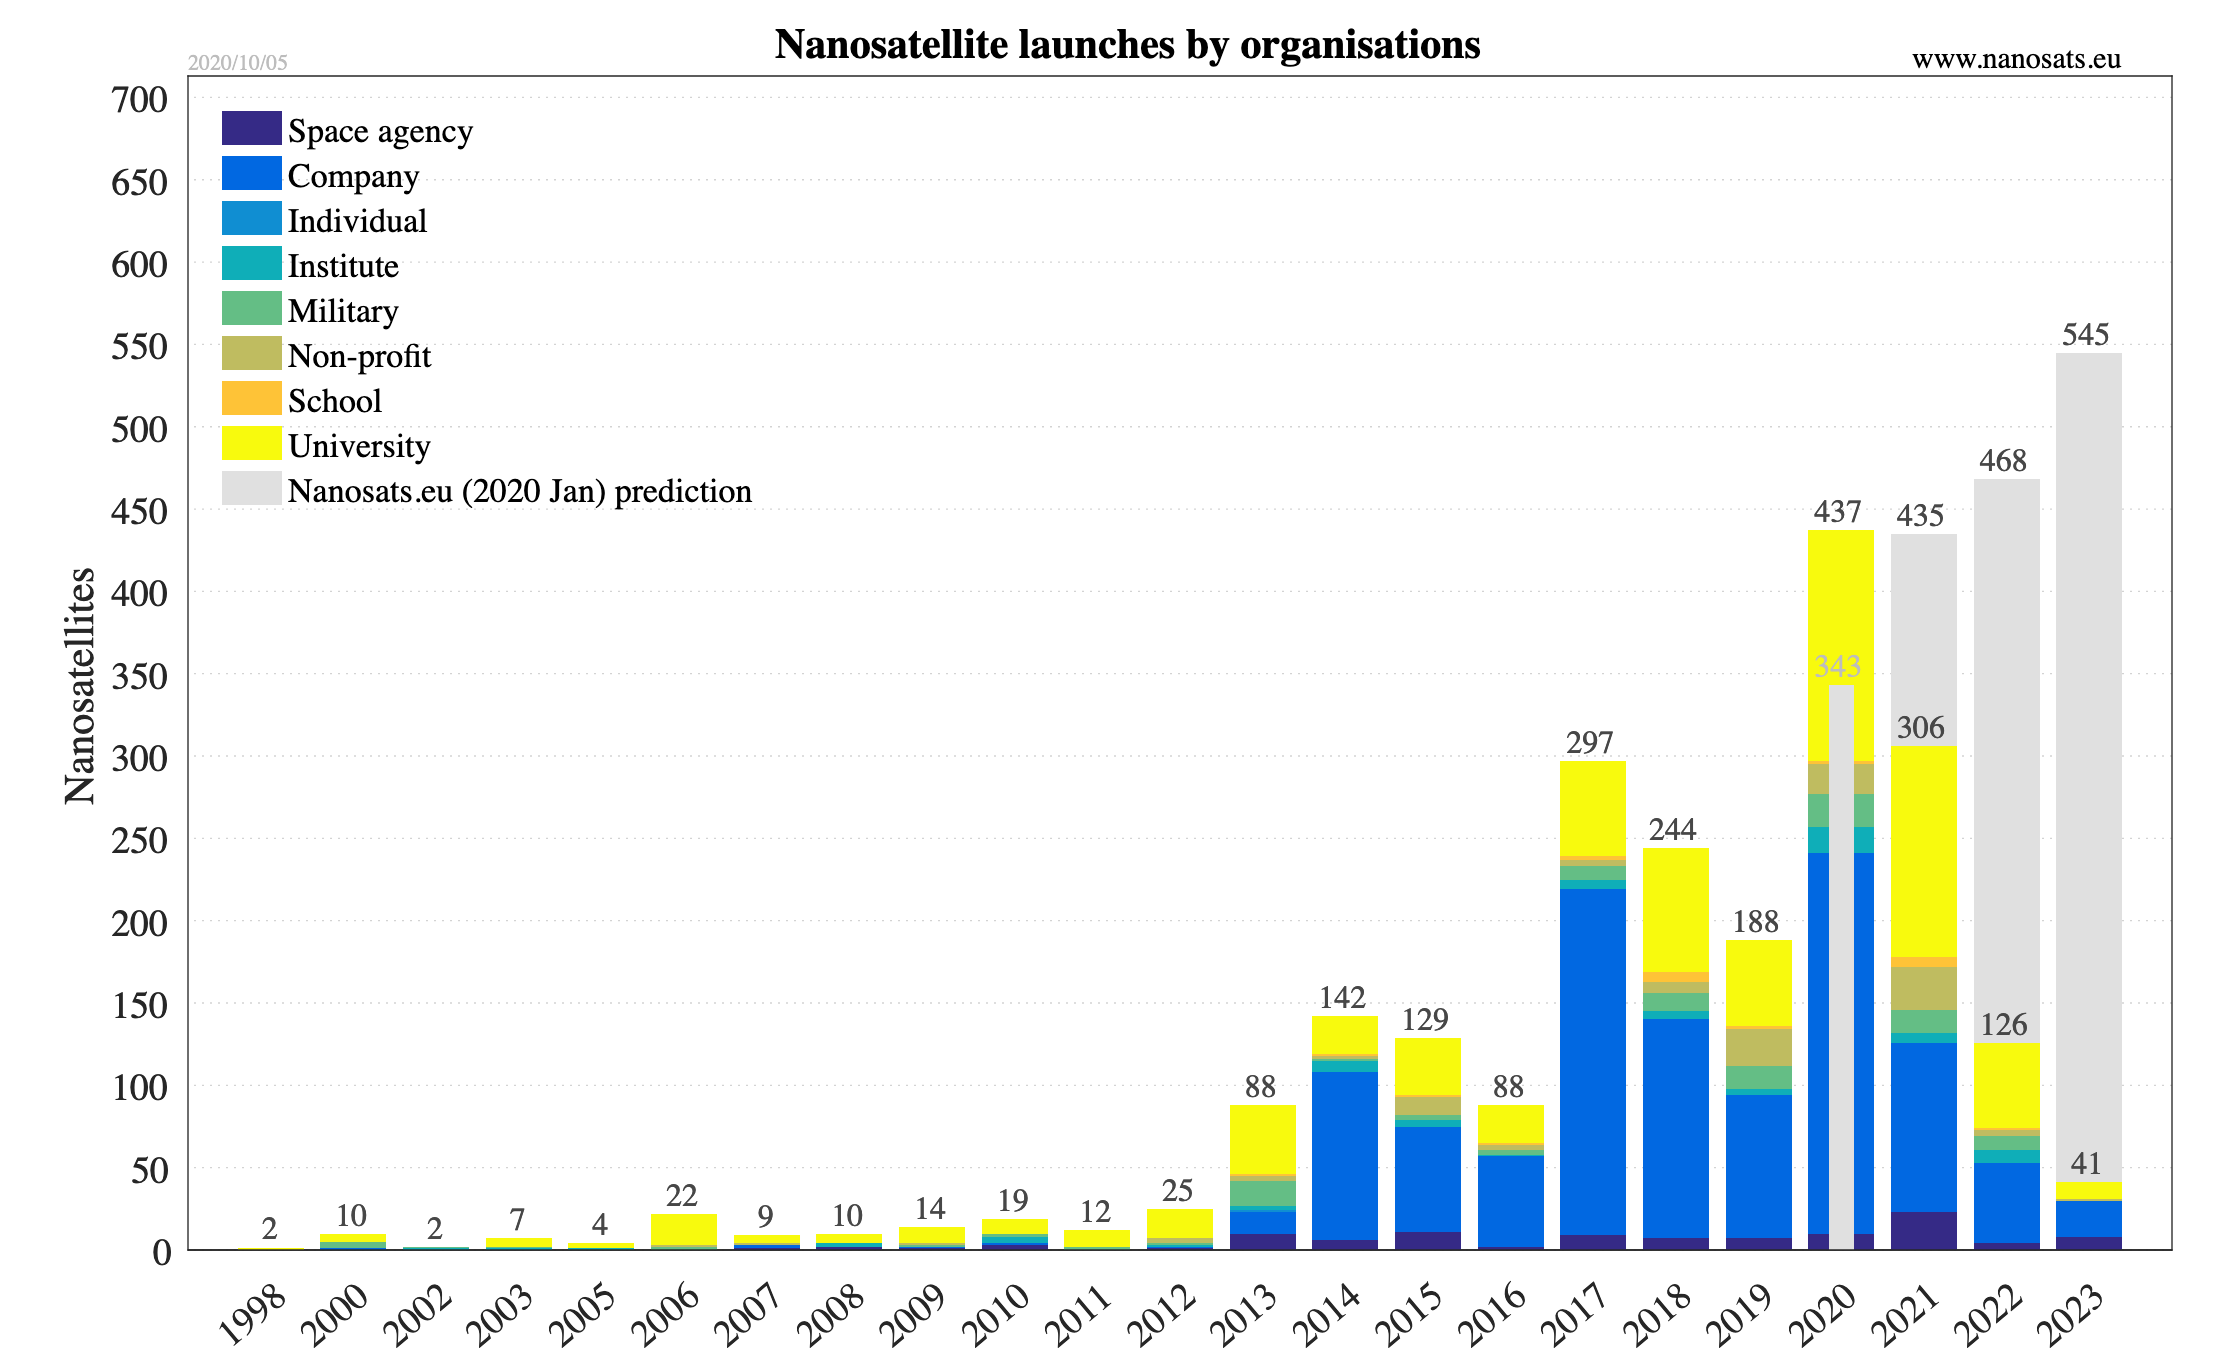
\includegraphics[width=\textwidth]{Thesis/Literature_Review/Lit Review Figures/launch institutions.png}
    \caption{CubeSat Development by Institution}
    \label{fig:CubeSat Development by Institution}
\end{figure}

\begin{figure}[H]
    \centering
    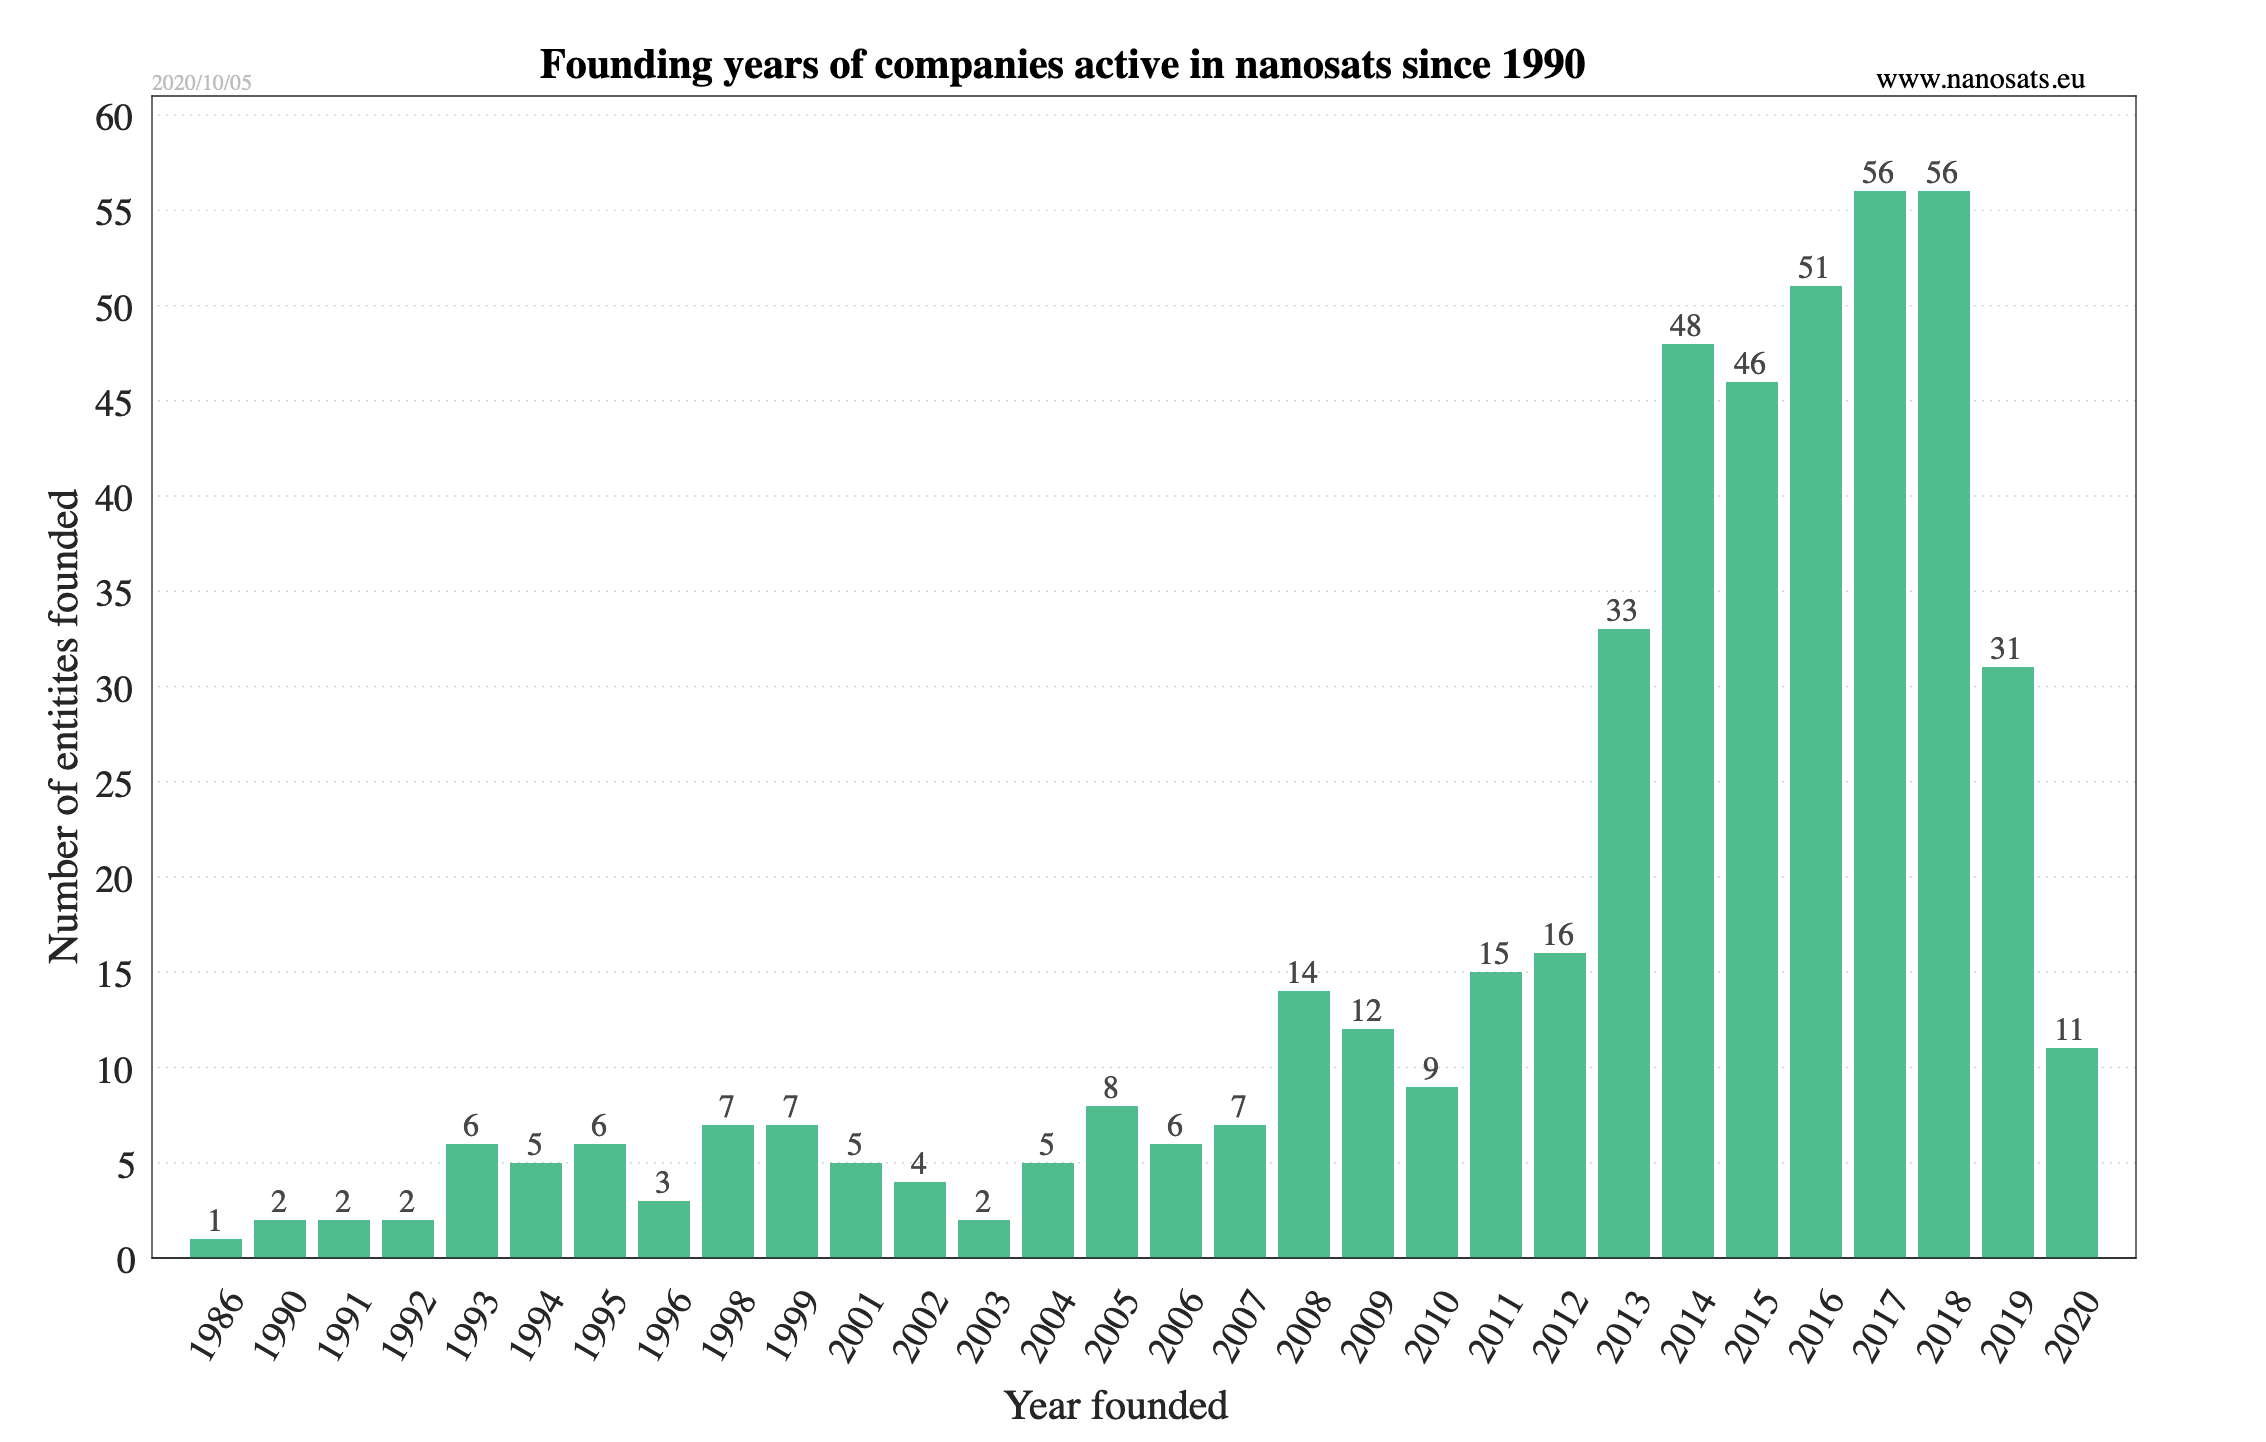
\includegraphics[width=\textwidth]{Thesis/Literature_Review/Lit Review Figures/CubeSat companies.png}
    \caption{CubeSat Companies}
    \label{fig:CubeSat Companies}
\end{figure}

Furthermore, as resiliency in space becomes more important, CubeSats offer a solution that is attracting research for military applications. As CubeSats are so small and affordable, a mission could include many individual CubeSats as a system, or "swarm," to create a large constellation that drastically increases the overall reliability and resiliency for the mission. In the private sector, a notable example is the Swarm SpaceBee, a 0.25U CubeSat that is part of a 150-CubeSat constellation in \abbreviationFull[Low Earth Orbit]{LEO}, testing out global \abbreviationFull[Internet of Things]{IOT} tracking of ships, vehicles, and other remote sensors \citep{Harris2019}. 

Finally, Launch Service Providers are routinely offering ride-share opportunities as secondary customers, making it much easier to launch these CubeSats in greater numbers. SpaceX launched SSO-A in 2018 which carried 15 microsatellites (10-100 kg) and 49 CubeSats, which came from universities and other research institutes from around the world including the previously mentioned FalconSat-6 \citep{eoPortal}. This CubeSat standard and the increasing demand for small satellites in orbit has lowered the barrier to entry, allowing universities and small research teams to develop their own space programs. In fact, AFIT has its own CubeSats in development, including the "Grissom" 6U bus, which will form the foundation for several distinct CubeSat variations.

Due to the unique advantages that CubeSats offer for both the Department of Defense and to small university teams, AFIT has embraced the concept and is preparing graduate students for future jobs in satellite acquisitions using CubeSats as the primary tool. Developing a CubeSat is a challenging task, especially for students without industry experience, so the MBSE method is first taught to students before applying it to CubeSat design.





